\documentclass[letterpaper,11pt]{article}

\usepackage{latexsym}
\usepackage[empty]{fullpage}
\usepackage{titlesec}
\usepackage{marvosym}
\usepackage[usenames,dvipsnames]{color}
\usepackage{verbatim}
\usepackage{enumitem}
\usepackage[hidelinks]{hyperref}
\usepackage{csquotes}
\usepackage[english]{babel}
\usepackage{graphicx}
\usepackage{multirow}
\usepackage{hanging}
\usepackage[style=geschichtsfrkl,sorting=none,maxnames=8]{biblatex}
\addbibresource{pubs.bib}

\newcommand{\nameuse}[1]{%
	\def\do##1{\settoggle{blx@use##1}{#1}}%
\dolistcsloop{blx@datamodel@names}}

% \pagestyle{fancy}
% \fancyhf{} % clear all header and footer fields
% \fancyfoot{}
% \renewcommand{\headrulewidth}{0pt}
% \renewcommand{\footrulewidth}{0pt}

% Adjust margins
\addtolength{\oddsidemargin}{-0.5in}
\addtolength{\evensidemargin}{-0.5in}
\addtolength{\textwidth}{1in}
\addtolength{\topmargin}{-.5in}
\addtolength{\textheight}{1.0in}

\urlstyle{same}

\raggedbottom
\raggedright
\setlength{\tabcolsep}{0in}

\newcommand{\rom}[1]{\uppercase\expandafter{\romannumeral #1\relax}}

% Sections formatting
\titleformat{\section}{
	\vspace{-4pt}\scshape\raggedright\large
}{}{0em}{}[\color{black}\titlerule \vspace{-5pt}]

%--------------------------------------
% Custom commands
\newcommand{\resumeItem}[2]{
\item\small{
		\textbf{#1}{: #2 \vspace{-2pt}}
	}
}
\newcommand{\resumeBullet}[1]{
\item\small{
		{#1 \vspace{-2pt}}
	}
}

\newcommand{\resumeSubheading}[5]{
	\vspace{-1pt}\item
	\begin{tabular*}{0.97\textwidth}[t]{ll@{\extracolsep{\fill}}r}
		\multirow{2}{*}{#1} & \textbf{#2} & #3 \\
				    & \textit{\small#4} & \textit{\small #5} \\
	\end{tabular*}\vspace{-5pt}
}

\newcommand{\resumeSubItem}[2]{\resumeItem{#1}{#2}\vspace{-4pt}}

\renewcommand{\labelitemii}{$\circ$}

\newcommand{\resumeSubHeadingListStart}{\begin{itemize}[leftmargin=*,label=]}
\newcommand{\resumeSubHeadingListEnd}{\end{itemize}}
\newcommand{\resumeItemListStart}{\begin{itemize}[label=$\bullet$]}
\newcommand{\resumeItemListEnd}{\end{itemize}\vspace{-5pt}}
%--------------------------------------

%%%%%%%%%%  CV STARTS HERE  %%%%%%%%%%%
\begin{document}

%--------------HEADING-----------------
\begin{tabular*}{\textwidth}{l@{\extracolsep{\fill}}r}
	\textbf{\href{http://dance.offinto.space}{\Large Daniel Nakhimovich}} & \href{dnahimov@gmail.com}{dnahimov@gmail.com}\\
	\href{http://dance.offinto.space}{\underline{http://dance.offinto.space}} & +1 551-795-5019 \\
\end{tabular*}
%--------------------------------------

%-------------EDUCATION----------------
\section{Education}
\resumeSubHeadingListStart
\resumeSubheading
{
\includegraphics[width=23pt]{./images/rutgers.png}}
{Rutgers University}{New Brunswick, NJ}
{Doctor of Philosophy in Computer Science \& Robotics; GPA: 3.97}{Sept 2019 -- May 2026}
\resumeSubheading
{
\includegraphics[width=23pt]{./images/cooper.png}}
{The Cooper Union}{New York, NY}
{Bachelor of Engineering in Electrical Engineering; GPA: 3.55}{Sept 2015 -- May 2019}
\resumeSubheading
{
\includegraphics[width=23pt]{./images/machonshlomo.png}}
{Machon Shlomo: The Heiden Institute}{Jerusalem, Israel}
{Jewish Law, Ethics, Philosophy, and Leadership}{Sept 2021 -- June 2023}
\resumeSubHeadingListEnd
%--------------------------------------

%------------PUBLICATIONS--------------
\section{Peer-Reviewed Publications}

\nocite{*}
\renewcommand*{\intitlepunct}{\addspace}
\DeclareFieldFormat{title}{\mkbibbold{#1}}
\DeclareFieldFormat{journaltitle}{\mkbibemph{#1\isdot}}
\DeclareFieldFormat{issuetitle}{\mkbibemph{#1}}
\DeclareFieldFormat{maintitle}{\mkbibemph{#1}}
\DeclareFieldFormat{booktitle}{\mkbibemph{#1}}
\nameuse{false}
\printbibliography[heading=none]

% \section{Upcoming Publications}
% \begin{hangparas}{.25in}{1}
% \textbf{Uniform Object Rearrangement: From Complete Monotone Primitives to Efficient Non-Monotone Informed Search}, by Rui Wang, Kai Gao, Daniel Nakhimovich, Jingjin Yu, and Kostas E. Bekris, submitted to \textit{IEEE International Conference on Robotics and Automation (ICRA)}, 2021.

% \vspace{0.1in}
% \textbf{Robotics as an Enabler of Resiliency to Disasters: Promises and Pitfalls}, by Rui Wang, Daniel Nakhimovich, Clinton J. Andrews, Fred Roberts, and Kostas E. Bekris, submitted to \textit{Lecture Notes in Computer Science / Lecture Notes in Artificial Intelligence (LNCS/LNAI)}, 2021.
% \end{hangparas}
% \vspace{0.2in}
%--------------------------------------

%--------------RESEARCH----------------
\section{Additional Research Projects}
\resumeSubHeadingListStart
\resumeSubheading
{
\includegraphics[width=23pt]{./images/pracsys.png}}
{PRACSYS}{New Brunswick, NJ}
{PI: Kostas Bekris}{Sept 2019 -- May 2025}
\resumeItemListStart
\resumeItem{Robot Nudging}
{A robot nudge is a robot behavious or ineherent design which alters a person's behaviour without significantly changing the incentive structure. I performed an extensive literature review of the subject in order to discover which ethical parameters are most urgent to consider for robot designers and policy makers.}
\resumeItem{Object Rotation Task Descriptions for Robots in English}
{I performed an informal survey, collecting human descriptions in English of household objects being rotated in a simulated environment. The goal is to study how people naturally describe tasks to a robot without using ``key words'' or ``wake phrases''.}
\resumeItem{Put That There}
{Human-Robot Interaction studies typically focus on robots understanding humans whereas this project studies how robots can be better understood by humans. I designed and performed expreriments to test human ability to interpret instructions given by a real robot.}
\resumeItemListEnd
\resumeSubheading
{
\includegraphics[width=23pt]{./images/dimacs.png}}
{DIMACS}{Piscataway, NJ}
{PI: James Abello}{Summer 2018 -- 2020}
\resumeItemListStart
\resumeItem{k-connectivity}
{k-connectivity is a connectivity measure for graphs. I designed two algorithms for finding approximations of minimum seperating sets of a graph in order to perform efficient graph decomposition for data visualization.}
\resumeItem{Graph Peeling}
{Graph Peeling is the iterative process of removing vertices from a graph. I explored properties of various graph peeling techniques and designed a new peeling algorithm (wave decomposition) in order to decompose very large graphs efficiently.}
\resumeItemListEnd
\resumeSubHeadingListEnd
%--------------------------------------

%--------------PROJECTS----------------
\section{One-off Projects}
\resumeSubHeadingListStart
\resumeSubItem{2019; OpenSesame}
{Open source cryptographic co-processor implemented on an FPGA}
\resumeSubItem{2018; pass2act}
{Passive to active sentence transformer built using spaCy's dependency tree parser}
\resumeSubItem{2017; biboch}
{Bitboard checkers implementation with an AI that performs a fast alpha/beta search on the game tree}
\resumeSubItem{2016; 8-bit processor}
{Custom 8-bit instruction set architecture written in verilog}
\resumeSubItem{2015; 2048 Circuit}
{A recreation of the popular mobile game 2048 using various CMOS ICs, buttons, and LEDs}
\resumeSubHeadingListEnd
%--------------------------------------

%--------------TEACHING----------------
\section{Teaching/Mentor Experience}
\resumeSubHeadingListStart
\resumeSubheading
{
\includegraphics[width=23pt]{./images/lumiere.png}}
{Lumiere Education}{Online}
{Research Mentor}{Summer 2023}
\resumeSubheading
{
\includegraphics[width=23pt]{./images/rutgers.png}}
{Rutgers University}{New Brunswick, NJ}
{Mentor to Undergraduate Students in Robotics}{2020 -- 2021}
\begin{tabular*}{0.97\textwidth}[t]{ll@{\extracolsep{\fill}}r}
	\vspace{-10pt}\\
	~~~~~~ & \textit{\small Teaching Assistant for \href{https://www.cs.rutgers.edu/academics/graduate/m-s-program/course-synopses/course-details/16-198-512-introduction-to-data-structures-and-algorithms}{Introduction to Data Structures and Algorithms}} & \textit{\small Fall 2019} \vspace{-10pt}\\
\end{tabular*}
\resumeSubheading
{
\includegraphics[width=23pt]{./images/conceptheca.png}}
{Conceptheca}{Fair Lawn, NJ}
{Mentor to Android Developement Interns}{2015 -- 2016}
\resumeSubheading
{
\includegraphics[width=23pt]{./images/fairlawn.png}}
{Fair Lawn High School}{Fair Lawn, NJ}
{Marching Band Woodwind Section Leader and Clarinet Tutor}{2014 -- 2015}
\resumeSubHeadingListEnd
%--------------------------------------

%-------------EXPERIENCE---------------
\section{Industry Experience}
\resumeSubHeadingListStart
\resumeSubheading
{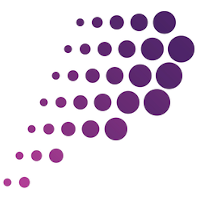
\includegraphics[width=23pt]{./images/pulsepoint.png}}
{PulsePoint}{New York, NY}
{TechOps Intern}{Summer 2017}
\resumeItemListStart
\resumeBullet{Reduced false positive QPS (queries per second) alerts by 92\% by filtering out statistical outliers.}
\resumeBullet{Implemented automated backups and data verification of ten 100GB databases using Bash scripts and SQL queries executed inside temporary Docker containers.}
\resumeBullet{Physically diagnosed and reconfigured 2 servers, ensuring continuous uptime of critical application infrastructure.}
\resumeBullet{Developed 3 new dashboards used for monitoring application reliability.}
\resumeItemListEnd

\resumeSubheading
{
\includegraphics[width=23pt]{./images/conceptheca.png}}
{Conceptheca}{Fair Lawn, NJ}
{Mobile Application Developer}{2015 -- 2016}
\resumeItemListStart
\resumeBullet{Identified key medical procedures, via collaborating with Doctors, that could use mobile applications to reduce a physician's workload 85\%.}
\resumeBullet{Designed and implemented 2 applications (Android and iOS) to aid medical professionals to better monitor patients and administer medication.}
\resumeBullet{Incorporated generative/procedural algorithms in a mobile application to create artistic high resolution images (4k) in less than 1 second.}
\resumeBullet{Incorporated generative algorithms in a mobile app to create abstract art.}
\resumeItemListEnd
\resumeSubHeadingListEnd
%--------------------------------------

%---------------SKILLS-----------------
\section{Skills}
\resumeSubHeadingListStart
\resumeSubItem{Programming Languages}
{C/C++, C\#, Python, Linux, Java, Rust, MATLAB, Verilog, Bash, PHP, SQL, Ruby}
\resumeSubItem{Software Libraries}{OpenCV, PyTorch, ROS, MuJoCo, Ollama, Unity, Docker, Boost, spaCy, MongoDB}
\resumeSubItem{Robots and Hardware}{Baxter, Yaskawa Motoman, Xilinx FPGAs, 3D Printers}
\resumeSubItem{Natural Languages}{English (Native), Russian (Conversant), Hebrew (Read Only)}
\resumeSubHeadingListEnd
%--------------------------------------

%---------------AWARDS-----------------
\section{Awards/Certifications}
\resumeSubHeadingListStart
\resumeSubItem{2023; Best Design Process Award at HRI}{Development of a Socially Cognizant Robotic Campus Guide}
\resumeSubItem{2023; Certificate in Socially Cognizant Robotics}{Upon completing 2 years in an NSF-funded National Research Traineeship focused on Socially Cognizant Robotics for a Technology Enhanced Society}
\resumeSubItem{2021; Best Paper Award at BigVis}{Graph Cities: Their Buildings, Waves, and Fragments}
\resumeSubItem{2018; HackCooper; $1^{st}$ prize}
{skEye Net - Wireless eye tracking / gaze estimation headset that works in realtime}
\resumeSubItem{2015 --- 2019; Half-tuition scholarship}{Merit scholarship from Cooper Union}
\resumeSubItem{2015 --- 2019; Innovators Merit Scholarship}{Merit scholarship from Cooper Union}
\resumeSubItem{2015; David Lee Memorial Scholarship}{For academic achievment and community service}
\resumeSubHeadingListEnd
%--------------------------------------

\section{Miscellaneous}
\resumeSubHeadingListStart
\resumeSubItem{Peer Reviewes}{2019 - ...}
\resumeItemListStart
\resumeItem{ISER}{International Symposium on Experimental Robotics}
\resumeItem{IROS}{Conference on Intelligent Robots and Systems}
\resumeItem{RSS}{Robotics: Science and Systems Conference}
\resumeItem{CoRL}{Conference on Robot Learning}
\resumeItem{ICRA}{International Conference on Robotics and Automation}
\resumeItem{ICAR}{International Conference on Advanced Robotics}
\resumeItem{RA-L}{IEEE Robotics and Automation Letters}
\resumeItem{BigVis}{Big Data Visual Exploration and Analytics Conference}

\resumeItemListEnd
\resumeSubHeadingListEnd

%------------AFFILIATIONS--------------
% \section{Organizations}
%         \resumeSubHeadingListStart
%                 \resumeSubItem{Rutgers Astronomical Society}
%                 {}
%         \resumeSubHeadingListEnd
%--------------------------------------

\end{document}
